


\documentclass[
a4paper,        % A4 papier
headsepline,    % Kopfzeile
footsepline     % Fusszeile
]{scrartcl}

\usepackage[T1]{fontenc}
\usepackage[utf8]{inputenc}
\usepackage[english]{babel}
\usepackage{mathpazo}


\usepackage{blindtext}
\usepackage{url}
\usepackage{caption}
\usepackage{subcaption}
\usepackage{placeins}
\usepackage{units}
\usepackage{amssymb}
\usepackage{amsmath} % Required for some math elements 
\usepackage{graphicx} % Required for the inclusion of images

\usepackage{paralist}                               % Listen mit speziellen Identifiern
\usepackage{mdwlist}                                % Listen ohne Zwischenzeilenabstand



% My commands
\newcommand{\myemph}[1]{ \emph{#1} }



% My Theorems
\newtheorem{bsp}{Beispiel}
\newtheorem{theo}{Theorem}
\newtheorem{defi}{Definition}
\newtheorem{koro}{Korollar}
\newtheorem{lemma}{Lemma}
\newtheorem{algo}{Algorithmus}
\newtheorem{bew}{Beweis}





\setcounter{secnumdepth}{2}                         % Numerierungtiefe
\hyphenation{}




\pagestyle{plain}
\pagenumbering{arabic}







\begin{document}

\title{TMA4280 -- Project 2}
\author{Maximilian Kieler}
\date{\today}

\maketitle


\section*{Introduction}

Aim of this project is the parallel implementation of a solver for the two dimensional poisson equation
\begin{equation}
	\Delta u(x,y) = -f(x,y).
\end{equation}
The method uses Fourier transform. Further descriptions of the method are given in \cite{script} and \cite{task}. The implementation is done with use of MPI and OpenMP. The basic structure is in the distributed memory model. On top there are some loop--parallelisations in the shared memory model. After the implementation we verify the algorithm for various number of processes and do an analysis of the parallel behaviour.



\section*{Question 1}

The implementation of the solver bases on the serial code \cite{script}. The parallelisation is achieved by distributing the $m \times m$--matrix row wise into almost equal sized $m \times q$--matrices with $q = \frac{m}{P}$. If $q$ is not an integer it will be rounded in the way that the last process will have a minor amount of rows $m - q \cdot P$. This makes the method as load balanced as possible.\footnote{In our case we have $m=2^k -1$. If the number of processes is a power of two, the last process have only one row less to compute then the others.} The DFT will be performed on single rows whose immediately will be put into its place in the sendbuffer. By using all to all broadcasting the processes exchange their data in order to perform the transposation of the matrix. Due to explicit loop collapsing one loses abstraction but achieve better performance\footnote{Todays compiler do this often by itself.}. The readability suffers due to this way of implementation. In addition to the distributed implementation some loops are parallelised by using OpenMP. The output is realized through MPI--IO as a binary file, but was not enabled during the following measurements. All of them were performed on Lille \cite{lille}. The code is compiled by using \path{mpicc} and \path{mpif90} based on \path{gcc 6.3.0} and OpenMPI. The \path{O2}--Optimisation and \path{fopenmp}--Flag are set.


\section*{Question 2}

We run the program on Lille with different system sizes and number of processes. To verify the program we run convergence tests with the function 
\begin{equation}
	f(x,y) = \sin(\pi x)\sin(2 \pi y).
\end{equation}
The error is computed with the maximum norm. We observe in Fig.~\ref{fig:size_err}\begin{figure}[h] 
  \centering
     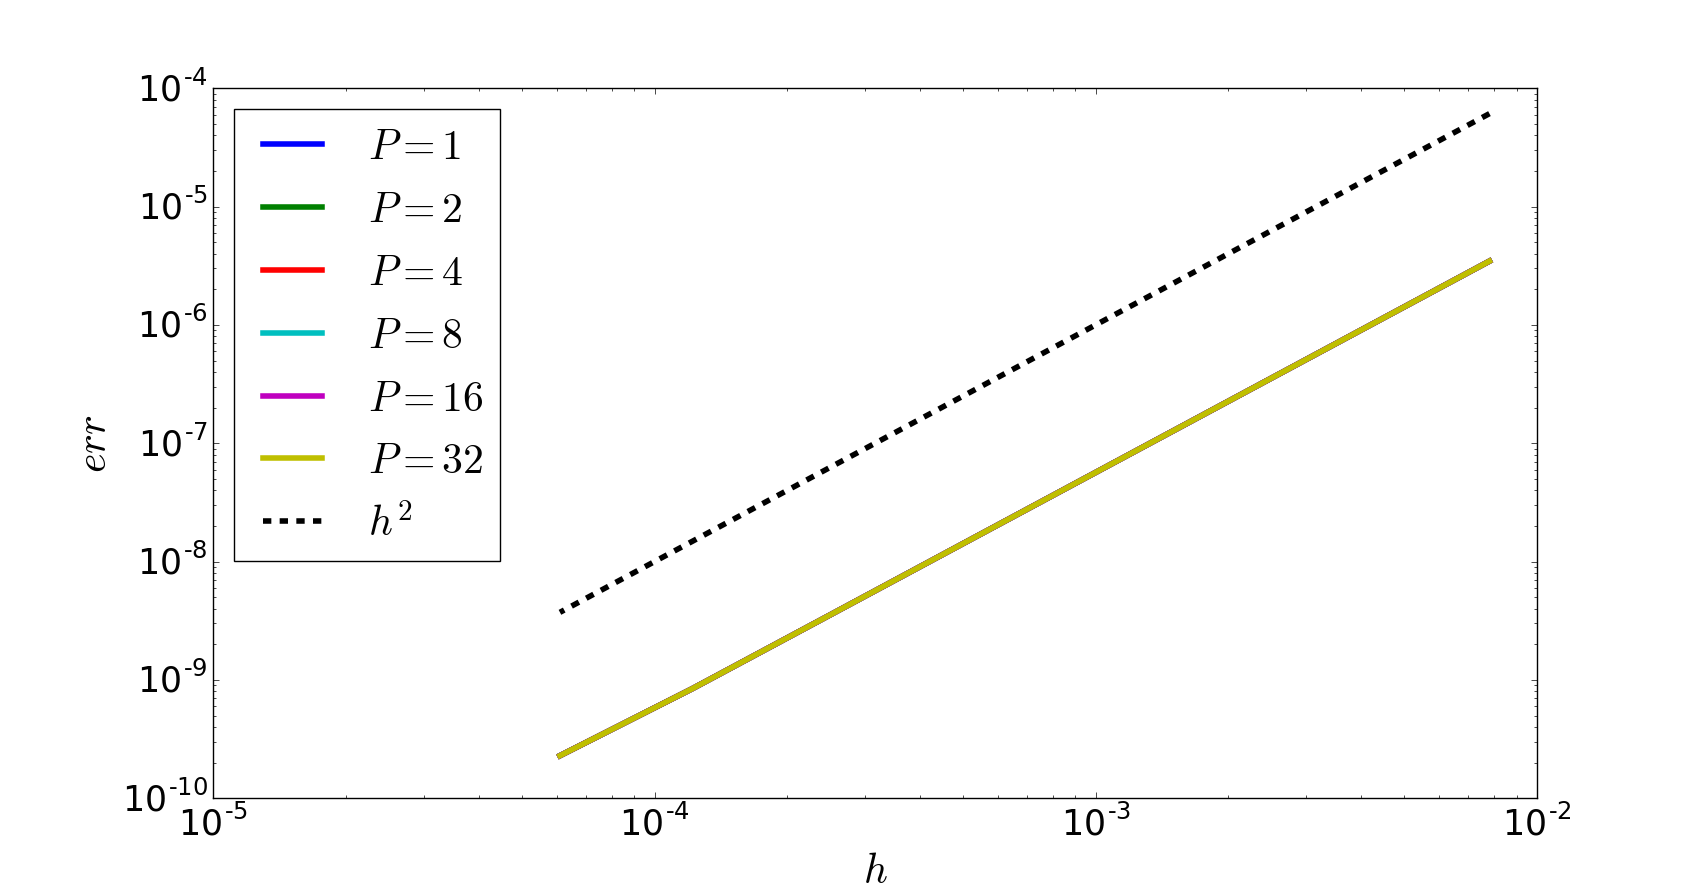
\includegraphics[width=\textwidth]{pic/size_err.png}
  \caption{Error of the method for different number of processes. Obvious there is almost no difference. The method works as expected.}
  \label{fig:size_err}
\end{figure} that the error decrease with the step size in order $2$ as we expect. This holds for different number of processes. Furthermore we measured the execution time of the program for different sizes $N$ and number of processes $P$. As we see in Fig.~\ref{fig:size_time}\begin{figure}[h] 
  \centering
     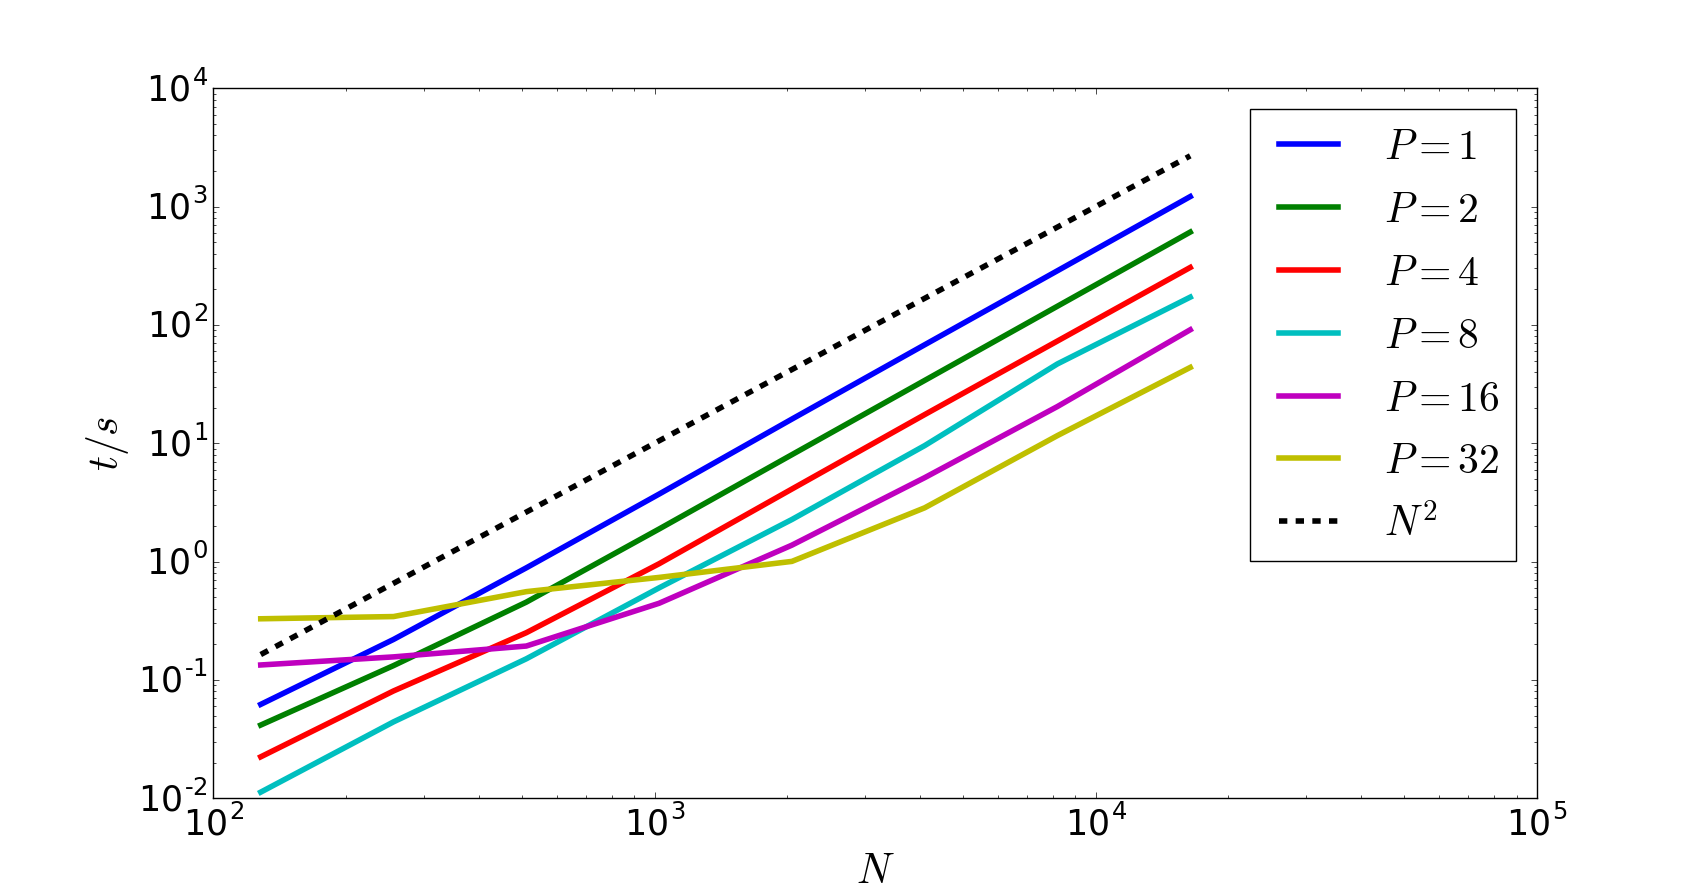
\includegraphics[width=\textwidth]{pic/size_time.png}
  \caption{The run time for different system sizes and number of processes. The runtime scales quadratic with the system size (logarithmic axis).}
  \label{fig:size_time}
\end{figure} the time increases quadratic in $N$. This is reasonable in reason that the system size increases with $N^2$. We observe for high numbers of processes and low $N$ a bad timing compared to runs with lesser processes, due to the higher communication overhead. 


\section*{Question 3}

We run the program for different choices of the number of MPI--Processes $P$ and OMP--Threads $T$. The condition $PT = 36$ is always satisfied. The results are depcited in \ref{fig:pt}\begin{figure}[h] 
  \centering
     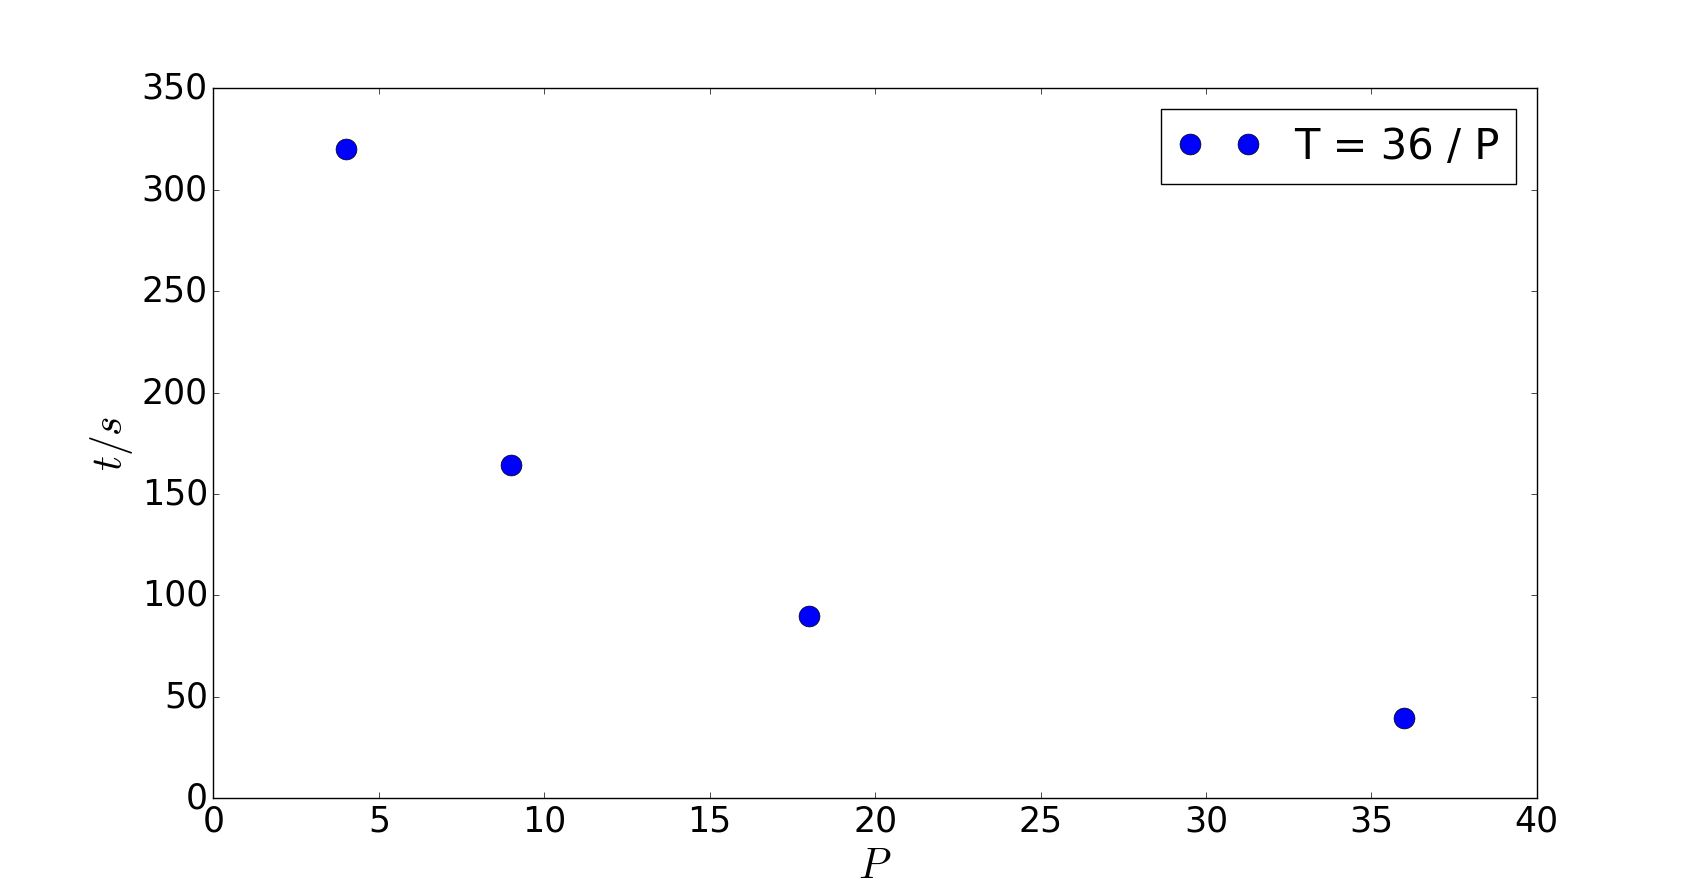
\includegraphics[width=\textwidth]{pic/pt.png}
  \caption{Runtime for different number of processes and threads for the system size $N = 2^14$.}
  \label{fig:pt}
\end{figure}. We do not observe a great improvement of the run time. This could be due to the possibility that the DFT is the most time consuming subtask of the algorithm. To support this assumption a more detailed analysis should be done.




\section*{Question 4}


In Fig.~\ref{fig:speedup}\begin{figure}[h] 
  \centering
     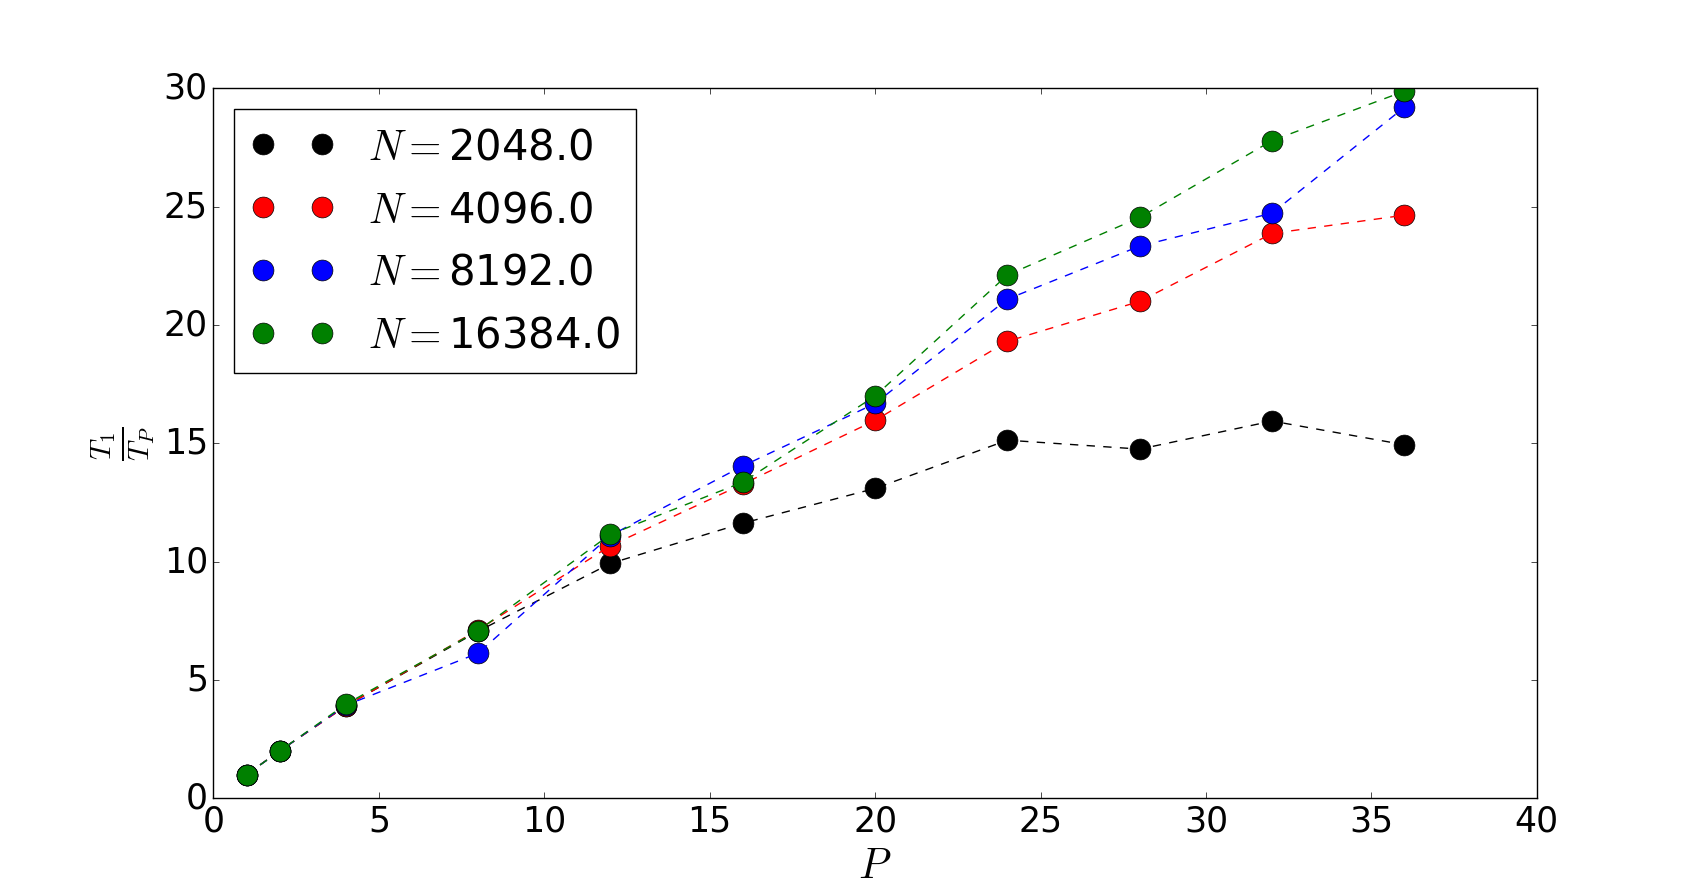
\includegraphics[width=\textwidth]{pic/speedup.png}
  \caption{The speed up for different system sizes. We see for small system sizes the speed up does not scale due to the increasing communication effort.}
  \label{fig:speedup}
\end{figure} the speed up is depicted for several sizes of the system. We observe especially for big sizes am almost ideal speed up. The efficency, depicted in Fig.~\ref{fig:efficency}\begin{figure}[h] 
  \centering
     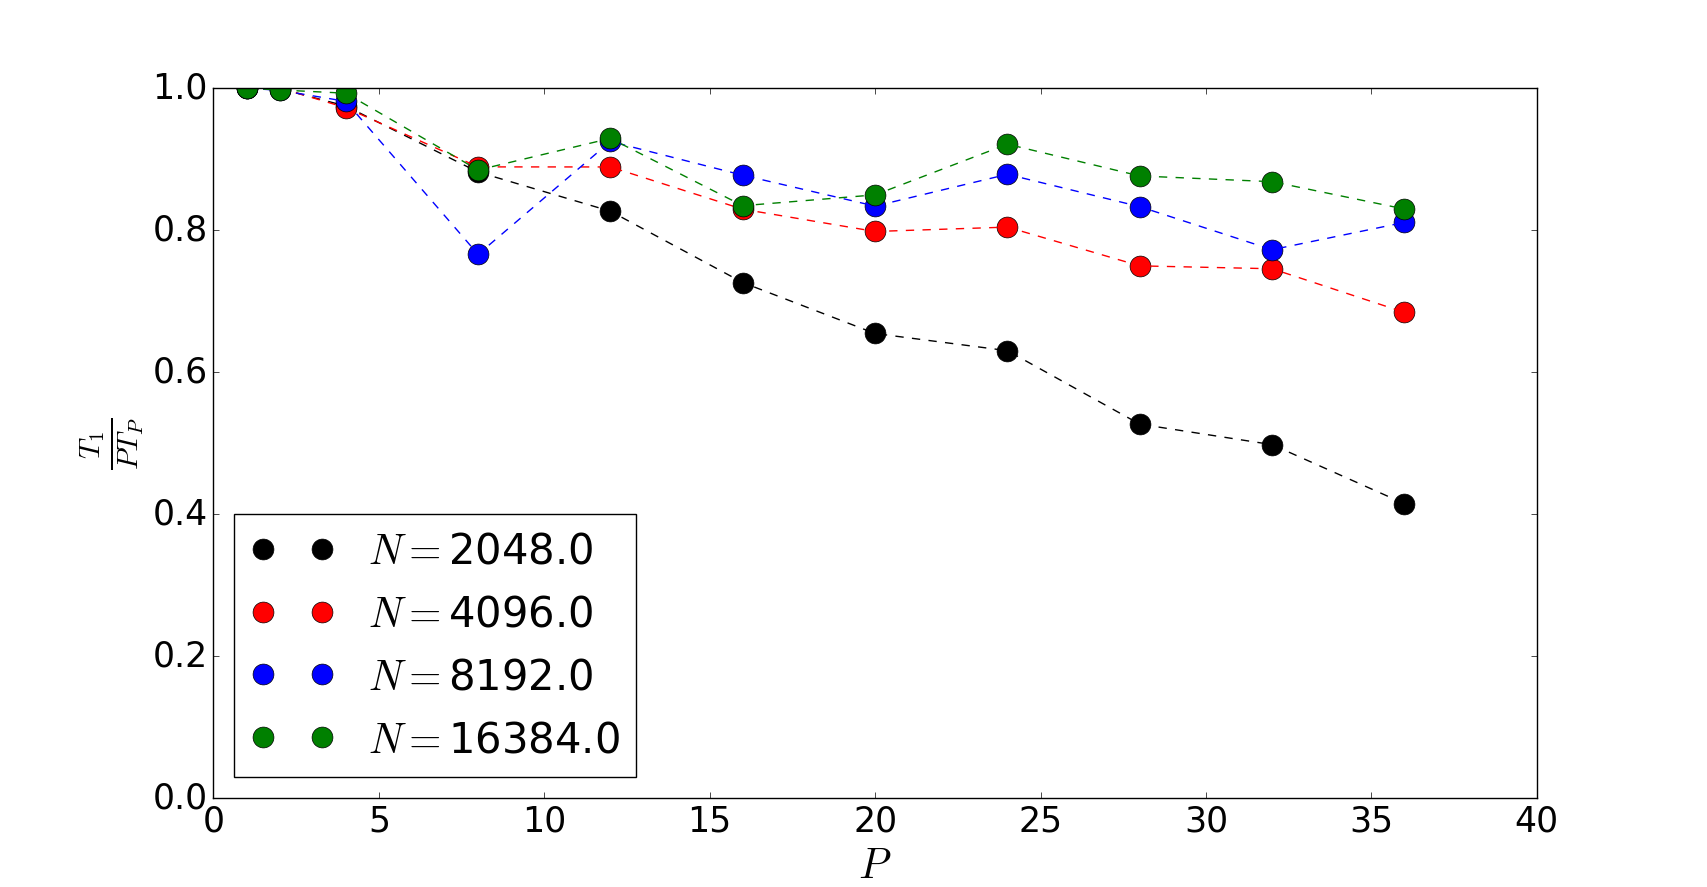
\includegraphics[width=\textwidth]{pic/efficency.png}
  \caption{The efficiency for different system sizes.}
  \label{fig:efficency}
\end{figure}, support this. Nevertheless we see that for smaller sizes of the system the communication overhead disturb the possible speed up. Due to Ahmdals law there is no advance in use more processes. But as we can suspect in Fig.\ref{fig:efficency} an increase of the system size and process number holds the efficiency almost constant. So our implementation is scalable. As previous mentioned the run time scales proportional to the system size with $N^2$. To improve the run time one can use more advanced implementation of the FFT. These algorithm runs faster if the size of the input is a power of $2$ unfortunately is the size of our input of size $2^k - 1$. One have to change this restriction to use more efficient a FFT. A possible bottleneck is the need of the transposation. The hole matrix is communicated at once and all processes can not continue before this data is transferred. Fortunately the system is almost load balanced. No process stays for long time idle. Instead of one communication after the FFT, one could pipeline the program in the way that after the of every single row this will be immediately communicated instead of buffering. But we assume that this leads to a higher communication overhead. In reason that we need all--t--all--broadcasting it should lead to improvements to use a suitable network for the processors. The expensive all--with--all--connection would minimize the time, but is for even big numbers of processors almost not realisable. one have to find a good compromise. 




\section*{Question 5}

We use as a new function
\begin{equation}
	f(x, y) = e^x \sin(2\pi x)\sin(2\pi y).
\end{equation}
The solution is depicted in Fig.~\ref{fig:func_plot}\begin{figure}[h] 
  \centering
     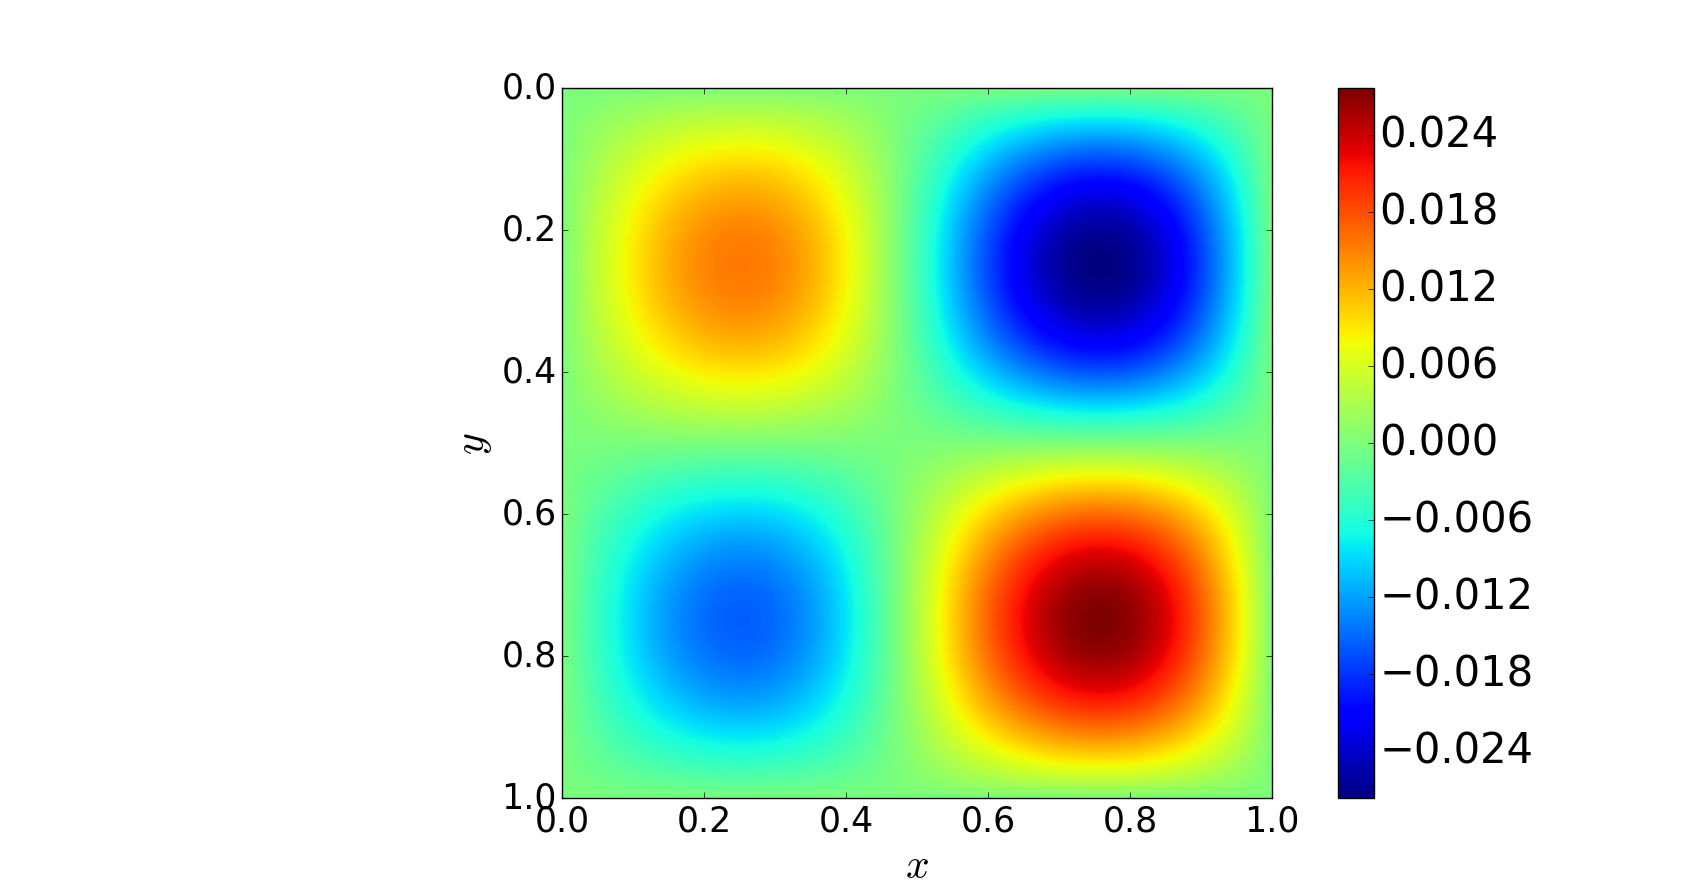
\includegraphics[width=\textwidth]{pic/func_plot.png}
  \caption{The solution for the given right hand function.}
  \label{fig:func_plot}
\end{figure}. In order to obtain results for different right hand functions we have not to change the parallel implementation scheme. Only the function which fill the right hand matrix have to be changed. Using built-in function like $\sin, \cos \ldots$ can increase the run time of the filling. But the main algorithm remains the same. One have of course to make sure that a solution of the problem exists and is unique.  

\section*{Question 6}

To implement the poisson problem with Dirichlet boundary condition we consider the discretised problem at the boundary nodes, i.e. $i = 1$
\begin{equation}
	-\frac{u_{i+1, j} - 2u_{i, j} + u_{i-1, j}}{h_x^2}  -\frac{u_{i, j+1} - 2u_{i, j} + u_{i, j-1}}{h_y^2} = f_{i,j}.
\end{equation}
Here is $u_{i-1, j} = u_{0, j}$ the constant value at the boundary. We add this term to the right hand function. This results in a poisson problem without boundary condition but with a modified right hand function. We can solve this problem with the same algorithm. However implementing von Neumann boundary conditions is more complicated in reason we have to change the left side of the equation and the size of the system.

\section*{Question 7}

By changing the size of the system we preserve number of nodes. We adjust $h_x = \frac{x_{max} - x_{min}}{n-1}$ and $h_y = \frac{y_{max} - y_{min}}{n-1}$. Hence we can write the problem as
\begin{equation}
	\frac{TU}{h_x^2} - \frac{UT}{h_y^2} = G.
\end{equation}
As a consequence the basic parallel implementation remains the same. Only the part of the eigenvalues have to me changed: $\frac{(d_i + d_j)}{h} \to \frac{d_i^x}{h_x^2} + \frac{d_j^y}{h_y^2}$. The eigenvalues $d$ have to be calculated twice for $x$ and $y$. Disadvantage of this method we get different accuracy in both directions. This means that we compute in one direction with more nodes than necessary. Other methods like FEM can handle such problems.


\section*{Conclusion}
We observed that this system is suitable for parallelism. It is scalable and nearly load balanced. Disadvantage is the need of an all--to--all--communication which is unavoidable. To achieve further improvements regarding run time it could be fruitful to do some research in analog computers \cite{ana_comp}. A combination of digital memory based computers with programmable analog computers on switchable integrated circuits could be lead to new improvements above the packing limit of transistor on a chip. But this is barley a comment on possibilities of a futuristic computer architecture. The future will show ho long Moore's law can hold.



\bibliographystyle{unsrt}
\bibliography{lit}



\end{document}